\documentclass{exam}
\usepackage{main}
\title{Contrôle}
\date{4 Décembre 2023}
\author{}

\qformat{\textbf{Exercice \thequestion :}\emph{(\thequestiontitle)\hfill}}

\begin{document}
\maketitle
\begin{questions}
\titledquestion{Motif en croix}
On construit des motifs à l'aide de jetons. Au départ, on dispose d'un seul jeton. Au fur et à mesure, on ajoute quatres jetons aux quatre points cardinaux afin de former une croix de plus en plus grande.
\begin{center}
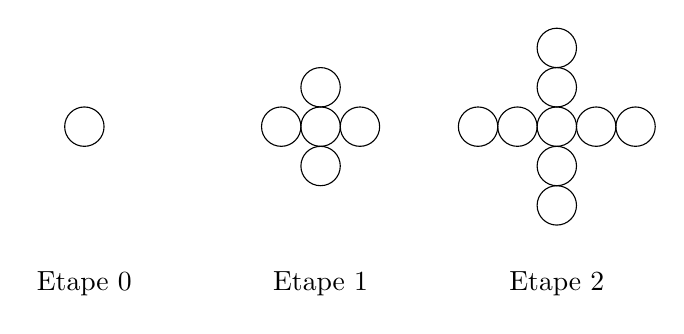
\begin{tikzpicture}
\draw (0,0) circle (0.25);
\draw (3,0) circle (0.25);
\draw (3.5,0) circle (0.25);
\draw (3,0.5) circle (0.25);
\draw (3,-0.5) circle (0.25);
\draw (2.5,0) circle (0.25);
\draw (6,0) circle (0.25);
\draw (6.5,0) circle (0.25);
\draw (7,0) circle (0.25);
\draw (5.5,0) circle (0.25);
\draw (5,0) circle (0.25);
\draw (6,0.5) circle (0.25);
\draw (6,1) circle (0.25);
\draw (6,-0.5) circle (0.25);
\draw (6,-1) circle (0.25);
\draw (0,-2) node {Etape $0$};
\draw (3,-2) node {Etape $1$};
\draw (6,-2) node {Etape $2$};
\end{tikzpicture}
\end{center}
\begin{parts}
\part On note $J_n$ le nombre de jetons utilisés à l'étape $n$. En utilisant la nature de la suite $(J_n)$, calculer le nombre de jetons à utiliser à l'étape $30$.
\part On remplace les jetons par des pièces de $50$ centimes. On note $E_n$ la somme en \euro{} nécessaire à l'étape $n$. Comment calculer $E_n$ en fonction de $J_n$ ? En déduire à partir de quelle étape a-t-on $50$ \euro{}. 
\end{parts}
\vspace{0.5cm}
\titledquestion{Intérêts composés}
Léon souhaite faire des économies. Pour cela, il place un capital de $2000$ \euro{} sur son livret A qui, sur la période considérée, propose un taux d'intérêts annuel de $0,75\%$. On suppose que ce taux reste inchangé dans les années qui suivent. Le livret A est un compte d'épargne rémunéré dont les intérêts cumulés sur l'année s'ajoute au capital en fin de chaque année.

Pour tout $n \in \N$, on note $C_n$ le capital en \euro{} disponible au bout de $n$ années de placement.
\begin{parts}
\part Calculer $C_0$, $C_1$ et $C_2$.
\part Justifier que la suite est géométrique et en préciser la raison.
\part Donner l'expression explicite de la suite $(C_n)$. Autrement dit, donner l'expression de $C_n$ en fonction de $n$.
\part À partir de combien d'années le capital de Léon dépasse les $3500$ \euro{} ?
\part Pour augmenter son capital, Léon décide de verser $500$ \euro{} sur son livret chaque année. On note $D_n$ son capital à l'année $n$, en prenant comme premier terme $D_0 = 2000$. Calculer $D_1$ et $D_2$.
\part Justifier que $(D_n)$ n'est ni arithmétique ni géométrique.  
\end{parts}
\vspace{0.5cm}
\titledquestion{Bonus}
Soit $(u_n)$ une suite arithmétique dont le premier terme est $3$, et dont le dixième terme est $22$. Quelle est la raison de cette suite ? Même question si la suite est géométrique. 
\end{questions}
\end{document}